\section*{Compiling Objects}

The dispatch problem occurs when the same interface is implemented by multiple classes. In the client program, it may be necessary to dynamically choose witch implementation to use. In order to do this, object contain a pointer to a \textbf{dispatch vector} (vtable) with pointer to method code. \medskip

For extension / inheritance, the dispatch vector gets extended at the end.\medskip
	
For multiple inheritance there are different approaches: 
\begin{compactitem}
	\item Allow multiple DV tables (C++), choose which DV to use based on static types, casting requires runtime operations.
			
	\item Use a level of indirection: Map method identifiers to code pointers using a hash table, search up through the class hierarchy.
			
	\item Give up separate compilation: Use sparse dispatch vectors or binary decision trees.
\end{compactitem}
	
Multiple Dispatch Vectors: Objects may have multiple entry points with individual DVs, casts change entry point of a variable
\vspace{-8pt}
\begin{center}
	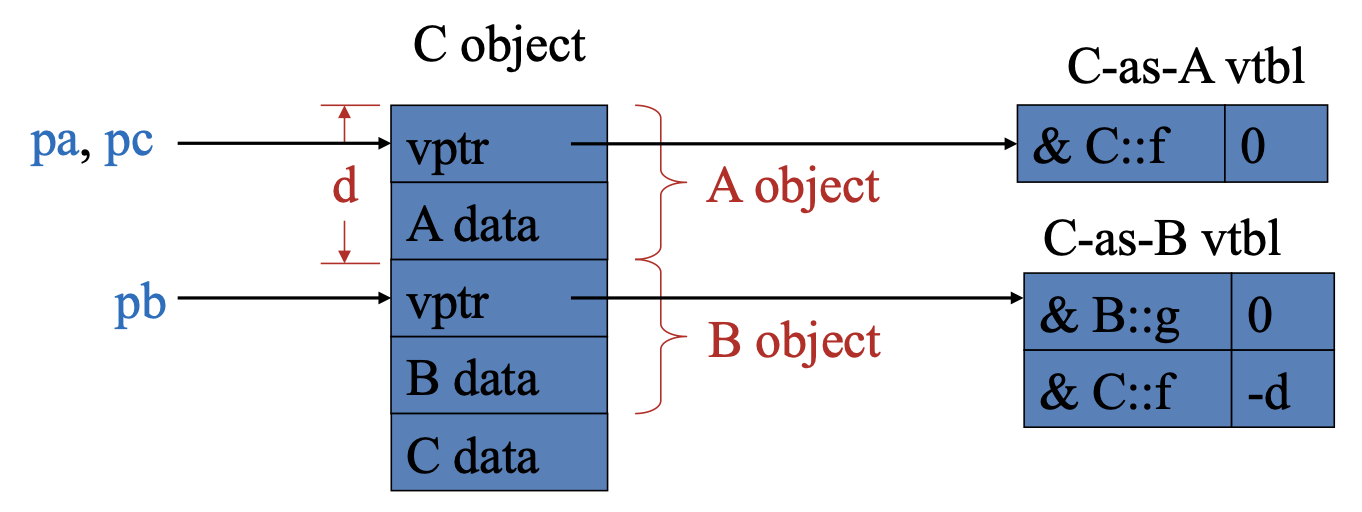
\includegraphics[width=0.7\linewidth]{vtable.png}
\end{center}
\vspace{-20pt}